\begin{figure}[!htbp]
  \begin{minipage}[t]{0.48\textwidth}
    \centering
    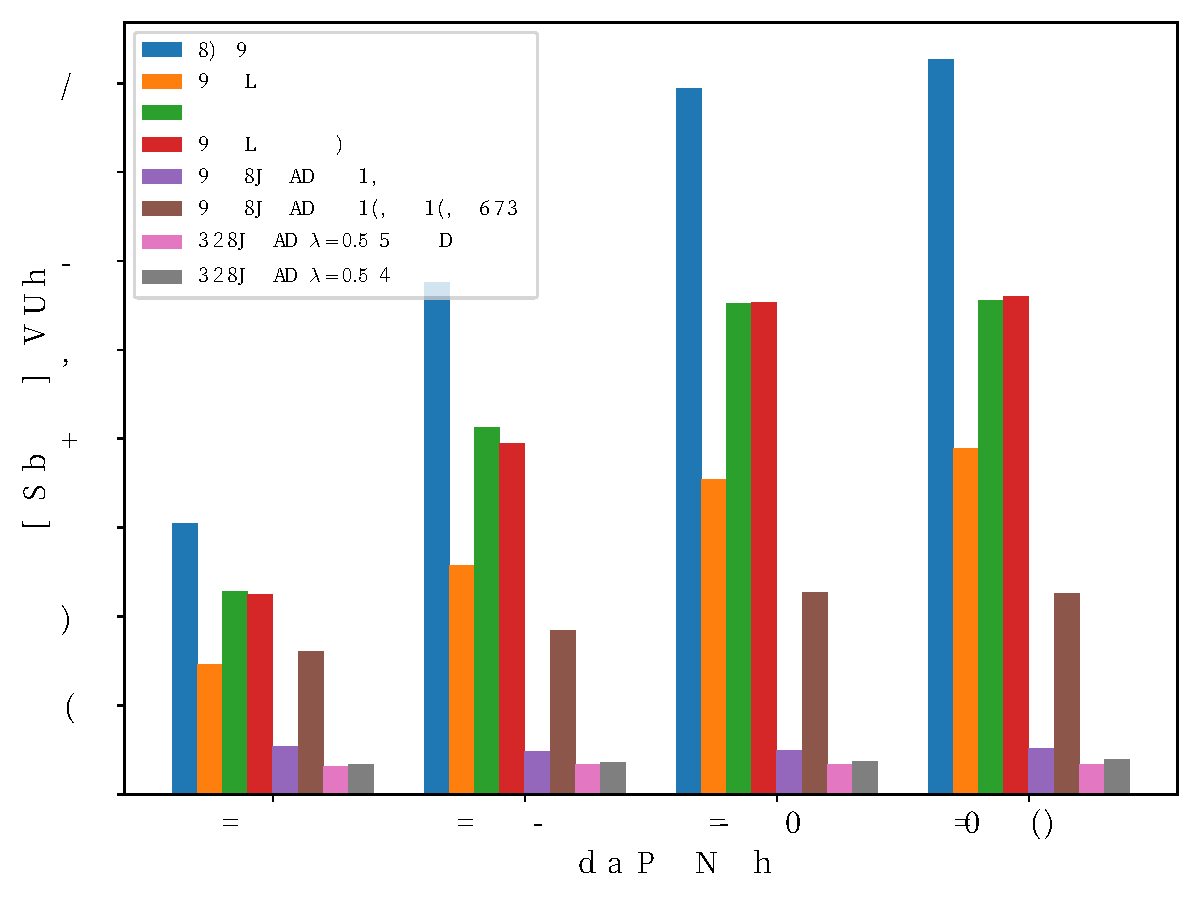
\includegraphics[width=\linewidth]{Img/decode_time.pdf}
    \bicaption{\enspace 不同源语音长度下各模型的翻译延迟对比。源语音按帧数分为4组，翻译延迟在单块RTX 3090 GPU上测试。}{\enspace Translation latency of different models across different source speech lengths, categorized into 4 groups based on source speech frame counts.}
    \label{fig:daspeech_decoding}
  \end{minipage}
  \hfill
  \begin{minipage}[t]{0.48\textwidth}
    \centering
    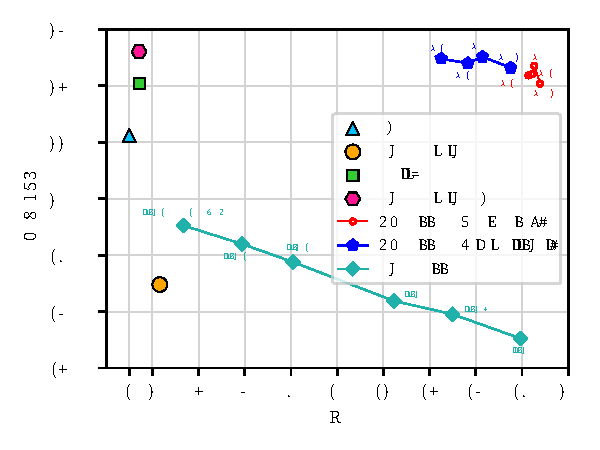
\includegraphics[width=\linewidth]{Img/tradeoff.pdf}
    \bicaption{\enspace 翻译质量与解码速度的权衡。横轴为相对于S2UT的加速比，纵轴为ASR-BLEU分数，右上方代表更好的权衡。}{\enspace Trade-off between translation quality and decoding speed. X-axis represents the speedup ratio relative to S2UT, and Y-axis represents ASR-BLEU.}
    \label{fig:daspeech_tradeoff}
  \end{minipage}
\end{figure}
